%\VignetteIndexEntry{GeneSelector Manual}
%\VignetteKeywords{Expression Analysis}
%\VignetteDepends{GeneSelector}
%\VignettePackage{GeneSelector}

\documentclass[a4paper, 11pt]{article}
%%% packages

%\usepackage{german}
%\usepackage[german]{babel}
\usepackage[latin1]{inputenc}
\usepackage{amsfonts}
\usepackage{amssymb}
\usepackage{amsmath}
\usepackage{amsthm}
\usepackage{latexsym}
\usepackage{verbatim}
\usepackage{epsfig}
\usepackage{fleqn}
\usepackage{color}
\usepackage[colorlinks=true, linkcolor=blue, anchorcolor=blue,
											citecolor=blue, filecolor=blue, menucolor=blue, pagecolor=blue,
											urlcolor=blue]{hyperref}
\usepackage{mathrsfs}
\usepackage{eufrak}
\usepackage{graphicx}
\usepackage{multicol}
\usepackage{amsbsy}
\usepackage{bm}
\usepackage[ruled]{algorithm2e}
\usepackage[nonamebreak,square]{natbib}
%\setcitestyle{authoryear,aysep={},yysep={;},numbers}

%%% page layout

\parindent0pt
\parskip1ex
\oddsidemargin-0.6cm
\evensidemargin-0.6cm
\topmargin-1cm
\textheight23cm
\textwidth15.1cm
\headsep0.5cm
\footskip0.5cm
%\usepackage{E:/R_Installation/share/texmf/Sweave}
\pagestyle{plain}

%%% Operators

\newcommand{\R}{{\mathbb R}}
\newcommand{\E}{{\mathbb E}}
\newcommand{\p}{{\mathbb P}}
\newcommand{\X}{{\mathcal X}}
\newcommand{\Y}{{\mathcal Y}}
\newcommand{\s}{{\mathscr S}}
\newcommand{\F}{{\mathscr F}}
\newcommand{\XX}{{\mathscr X}}
\newcommand{\h}{{\mathcal H}}
\newcommand{\LL}{{\mathcal L}}
\DeclareMathOperator*{\var}{var}
\DeclareMathOperator*{\cov}{cov}
\DeclareMathOperator*{\tr}{tr}
\DeclareMathOperator*{\diag}{diag}
\providecommand{\norm}[1]{\lVert#1\rVert}
\providecommand{\sp}{\langle \cdot, \cdot \rangle}
\providecommand{\M}[1]{\textbf#1}
\providecommand{\B}[1]{\bm#1}
\providecommand{\T}{\top}
\newcommand{\sign}{\operatorname{sign}}

\def\su{\sum_{i=1}^n}
\def\etall{\mbox{{\it et al., }}}
\def\etal{\mbox{{\it et al. }}}
\newcommand{\blanco}[1]{  }




\title{\large{\texttt{GeneSelector}} package vignette}
\author{Martin Slawski \footnote{\url{Martin.Slawski@campus.lmu.de}}\\
        Anne-Laure Boulesteix \footnote{\url{http://www.slcmsr.net/boulesteix}}}

\usepackage{e:/R_installation/share/texmf/Sweave}
\begin{document}
\date{\normalsize{Sylvia Lawry Centre, Hohenlindenerstr. 1, D-81677 Munich, Germany}}
\maketitle


\section{Statistical and Bioinformatical background}

One of the most important aspects of microarray data analysis is
the detection of genes that are differentially expressed, e.g., in different
experimental conditions or in individuals with different phenotypes.
The results of microarray studies are usually the starting point
for further more expensive and time-consuming experiments, which involve only a small number
of candidate genes that turned out to be 'most promising' in the previous step \citet{aer2006}.
Considering the induced efforts and costs, finding an accurate ranking of genes that
reduces the fraction of false positives under the top-ranking genes is a
crucial challenge in microarray data analysis.

The name \texttt{GeneSelector} refers to the following filter mechanism:
Starting from a large set of candidate genes, it stepwise excludes
more and more genes until one ends up with a very sparse set, called
'selected' genes. Its elements have the following property. Given some
threshold rank that is still considered biologically relevant,
the ranks of the selected genes are better than or at least equal to the threshold in all rankings performed
using different methods and different perturbed data sets. In a word,
they are consistently identified as differentially expressed.

Several rankings are generated using two approaches. On the one hand, the
original dataset is slightly perturbed, by randomly leaving one- or several
array(s) out, adding noise or swapping class labels. This procedure is repeated
many times. On the other hand,
one can use several ranking methods or test statistics - the current
implementation now features fifteen different procedures, including both traditional
and modern approaches (see an overview in Section 2).
The first approach tries to mimic a changed data situation and is therefore
helpful for assessing stability of the results (\citet{Pavlidis1}, \citet{Qiu}), while the
second one follows the spirit of a 'sensitivity analysis'. Almost all of the
considered test statistics rely on idealized assumptions and it is hard to check
whether they hold for a particular dataset at hand. In this context, using several
statistics is beneficial.

Furthermore, a major topic in \texttt{GeneSelector} is stability. If results tremendously
change when the data are slightly perturbed, they are little credible. We thank
In fact, microarray data are suspected to yield 'noise discovery' \citet{Ioannidis:noisy}.
To gain insight into stability, \texttt{GeneSelector} computes several
stability measures as discussed in the diploma thesis of Elisabeth
Gnatowski with the title 'Stability of methods for the analysis of differential
gene expression' \citet{Gnatowski2007} which served as a starting point in the
development of \texttt{GeneSelector}.

Let $\bm{X}=(x_{ji})_{\substack{j=1,\ldots,p \\ i=1,\ldots,n}}$ denote the matrix
of gene expression values (relative or absolute intensity values)
and  $\bm{y}=(y_i)$ the vector of class labels with
indices $i=1,\ldots,n$ for the observations (arrays) and $j=1,\ldots,p$
for the genes. For notational convenience, we set $\mathcal{D}=(\bm{X}, \bm{y})$.
All the procedures considered here
 return a triple \hypertarget{procedure}{$t(\mathcal{D})=(\bm{s}, \bm{p}, \bm{r})$}, where
\begin{itemize}
\item $\bm{s}$ is a $p \times 1$ vector of test statistics for each gene,
\item $\bm{p}$  is the corresponding vector of p-values given
      the statistic provides one,
\item $\bm{r}$ is a vector of \emph{ranks} for each gene, where rank 1
      is attributed to the gene being 'most distant' from the null
      hypothesis, i.e. most differentially expressed.
\end{itemize}
In this context, $t(\cdot)$ can in general be applied to the
independent two-sample case, the paired two-sample case and the one-sample
case.\\
In the \texttt{GeneSelector} package, the focus is on the ranks $\bm{r}$. The idea
behind \texttt{GeneSelector} is to exclude as many genes as possible
from the subset of candidate genes for differential expression, in order
to avoid false positives. {\it selected} genes
are those present at the top of the ranking with various featured procedures
$t(\cdot)$ as well as with $B$ {\it perturbed} data sets, which are denoted as
$\{\widetilde{\mathcal{D}}\}_{b=1}^B$. The \texttt{GeneSelector} package creates
perturbed data sets in order to take the stability of the findings into account.
By 'perturbed data sets' we mean data sets that
result from
\begin{itemize}
\item leaving out samples,
\item swapping class labels ($\widetilde{\bm{X}}=\bm{X}$),
      but $\bm{y}$ changes),
\item generating bootstrap replicates,
\item adding noise.
\end{itemize}
Results from 'perturbed' data sets and original dataset ($\mathcal{D}$) can be
aggregated in \texttt{GeneSelector} (separately for each different procedure)
in two ways (s. below), obtaining an aggregated ranking
$\bm{r}^{\text{agg}}(\mathcal{D}; t(\cdot))$.
After defining (or determining) some \hypertarget{thres}{'threshold rank'}
$1 \leq \theta \ll p$, the
\hypertarget{gk}{\texttt{GeneSelector}} procedure can be stated as follows:
\begin{enumerate}
\item Choose a set of test procedures for differential expressions
      $\{ t_k(.) \}_{k=1}^K$. For instance, one may choose $t_1(.)$ as the
ordinary t-test procedure and $t_2(.)$ as the foldchange procedure.
\item Apply each $t_k(.)$ to the original dataset $\mathcal{D}$ and to
      different perturbed data sets $\{ \widetilde{\mathcal{D}}_b \}_{b=1}^B$
\item Aggregate the resulting rankings to obtain
      $\bm{r}_k^{\text{agg}}, \; k=1,\ldots,K$.
\item Define an \hypertarget{orderstat}{order} on the set of test procedures
      $t_{(1)},\ldots,t_{(K)}$ so that $t_{(1)}$ is attributed
      most importance, $t_{(2)}$ second most and so on.
\item The final ranking follows now the following criteria
      \begin{itemize}
      \item[(1)] 'Selection' in $t_{(1)}$
      \item[$\vdots$]
      \item[(K)]  'Selection' in $t_{(K)}$
      \item[(K+1)] Rank in $t_{(1)}$
      \item[$\vdots$]
      \item[(2K)]  Rank in $t_{(K)}$
      \end{itemize}
      where 'Selection' means that the respective rank is below $\theta$
\end{enumerate}
The parameter $\theta$ can be interpreted as the highest rank one is
still interested in. For instance, if one expects 10 differentially
expressed genes, $\theta$ could be set to that value, but it should
usually taken higher, because the procedure outlined above will normally produce
less 'selected' genes than $\theta$.\\
Admittedly, the choice of $\theta$ is not easy. One possibilty of
finding this value adaptively consists of using multiple testing procedures
(s. example below).

\hypertarget{statisticsoverview}{\section{Overview of featured test procedures}}
There is a vast literature about test statistics to be used in the microarray
setting. Here, we provide a selection of 15 procedures. Of course, this selection
is non-exhaustive, but we have tried to include a good 'mixture'
of (sometimes completely different) approaches. They can be categorized in
the following way (the names of the corresponding functions implementing them are
written in typewriter):
\begin{itemize}
\item the naive approaches: Foldchange (\texttt{RankingFC}), a 'gap' statistic
      (\texttt{RankingGap})
\item 'ordinary' statistics: (usual) t-statistic (\texttt{RankingTstat}),
       Welch statistic (\texttt{RankingWelch}), Wilcoxon statistic
       (\texttt{RankingWilcoxon})
\item hierarchical bayesian models: Baldi-Long t-statistic
      (\texttt{RankingBaldiLong}, \citet{BaldiLong}),
      Fox-Dimmic t-statistic (\texttt{RankingFoxDimmic}, \citet{FoxDimmic}),
      the B-statistic (\texttt{RankingBstat}, \citet{Loennstedt}),
      'moderated' t-statistic (\texttt{RankingLimma}, \citet{Smyth})
\item two mixture model approaches named \texttt{RankingEbam} and
      \texttt{RankingWilcEbam}, respectively
      (\citet{Efron1}; \citet{Efron2}) that are
      connected with Significance Analysis for Microarrays
      (SAM, \citet{Tusher}) that is also included (\texttt{RankingSam}).
\item permutation-based t-statistics (\texttt{RankingPermutation})
\item 'modified' t-statistics: shrinkage t-statistic
      (\texttt{RankingShrinkageT}, \citet{st}), soft-threshold
       t-statistic (\texttt{RankingSoftthresholdT}, \citet{softt})
\end{itemize}


\section{An artifical dataset example}
\subsection{Generating the data set}
For demonstration purposes, we use a simulated datsets containing $2,000$
genes. It can be characterized in the following manner.
\begin{itemize}
\item $\bm{X}$ is drawn from a multivariate normal distribution
      with zero mean vector and covariance matrix $\bm{\Sigma}$.
\item $\bm{\Sigma}$ is drawn randomly from an Inverse Wishart
      distribution.
\item $\bm{y}$ consists of ten samples for each class, in the
      following regarded as two independent samples.
\item The first 40 genes (rows) of $\bm{X}$ are differentially
      expressed, where the differences $\Delta_j, j=1,\ldots,40$
      in mean between the two classes were simulated independently
      according to a normal distribution with variance 0.9.
\end{itemize}
We access the data using the lines:
\begin{Schunk}
\begin{Sinput}
> data(toydata)
> yy <- as.numeric(toydata[1, ])
> xx <- as.matrix(toydata[-1, ])
> dim(xx)
\end{Sinput}
\begin{Soutput}
[1] 2000   20
\end{Soutput}
\begin{Sinput}
> table(yy)
\end{Sinput}
\begin{Soutput}
yy
 1  2 
10 10 
\end{Soutput}
\end{Schunk}


Knowing that the first genes are actually differentially expressed, we make
boxplots of the first four genes:

\begin{Schunk}
\begin{Sinput}
> par(mfrow = c(2, 2))
> for (i in 1:4) boxplot(xx[i, ] ~ yy, main = paste("Gene", i))
\end{Sinput}
\end{Schunk}
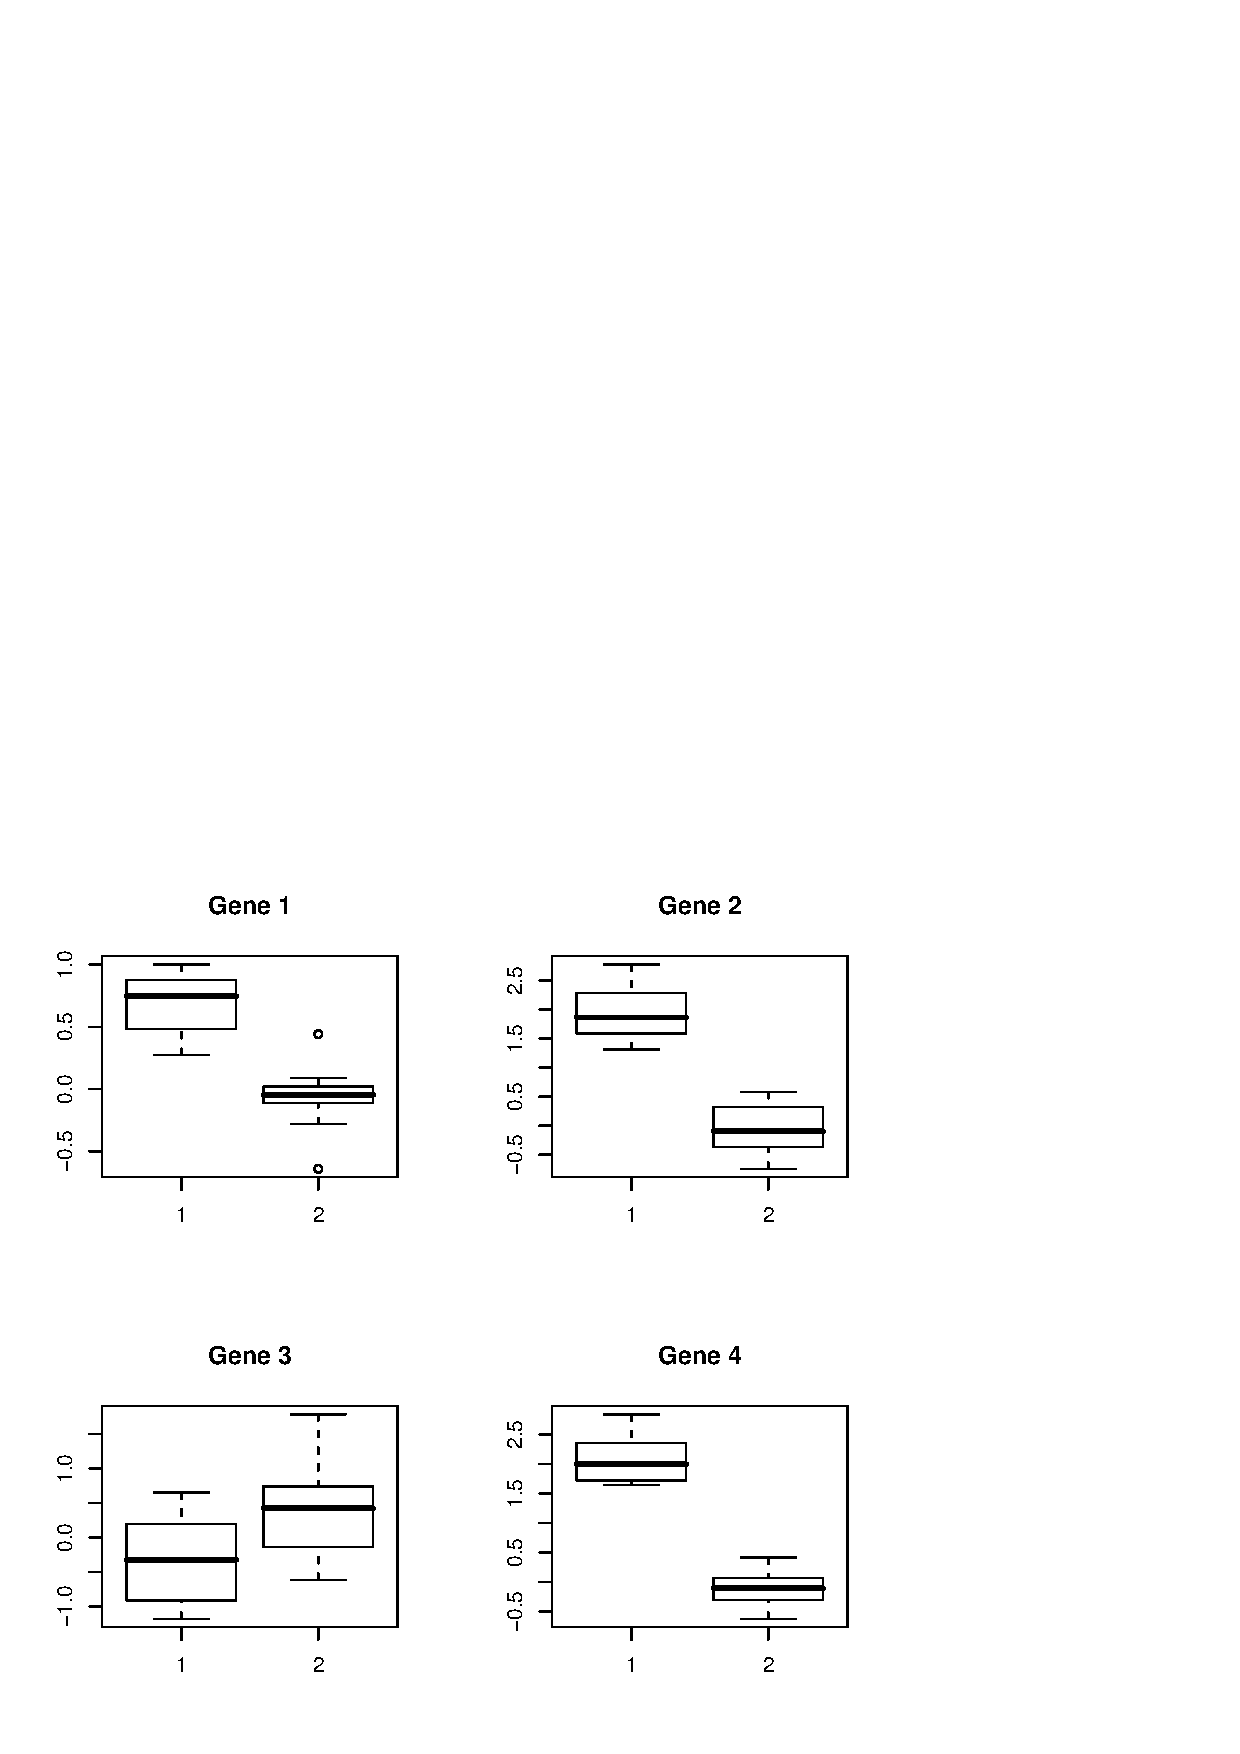
\includegraphics{GeneSelector-003}



\subsection{Ranking the genes}

We now peform 6 rankings from six methods:
\texttt{ordinaryT} (ordinary t-test), \texttt{BaldiLongT} (Baldi-Long t-statistic),
\texttt{FoxDimmicT} (Fox-Dimmic t-statistic),
\texttt{SAM}, \texttt{Wilcoxon}, \texttt{WilcEbam} and a modified version
of the Wilcoxon statistic derived from a mixture model.

\begin{Schunk}
\begin{Sinput}
> ordT <- RankingTstat(xx, yy, type = "unpaired")
> BaldiLongT <- RankingBaldiLong(xx, yy, type = "unpaired")
> FoxDimmicT <- RankingFoxDimmic(xx, yy, type = "unpaired")
> sam <- RankingSam(xx, yy, type = "unpaired")
> wilcox <- RankingWilcoxon(xx, yy, type = "unpaired", pvalues = TRUE)
> wilcoxefron <- RankingWilcEbam(xx, yy, type = "unpaired")
\end{Sinput}
\end{Schunk}

The resulting objects are all instances of the class \texttt{GeneSelector}.\\
To get some class information, we use the commands:

\begin{Schunk}
\begin{Sinput}
> class(ordT)
\end{Sinput}
\begin{Soutput}
[1] "GeneRanking"
attr(,"package")
[1] "GeneSelector"
\end{Soutput}
\begin{Sinput}
> getSlots("GeneRanking")
\end{Sinput}
\begin{Soutput}
          x           y   statistic     ranking        pval        type 
   "matrix"    "factor"   "numeric"   "numeric"    "vector" "character" 
     method 
"character" 
\end{Soutput}
\begin{Sinput}
> str(ordT)
\end{Sinput}
\begin{Soutput}
Formal class 'GeneRanking' [package "GeneSelector"] with 7 slots
  ..@ x        : num [1:2000, 1:20]  1.00  2.78 -1.18  2.79 -2.95 ...
  .. ..- attr(*, "dimnames")=List of 2
  .. .. ..$ : chr [1:2000] "1" "2" "3" "4" ...
  .. .. ..$ : chr [1:20] "arr1" "arr2" "arr3" "arr4" ...
  ..@ y        : Factor w/ 2 levels "1","2": 1 1 1 1 1 1 1 1 1 1 ...
  ..@ statistic: Named num [1:2000] 13.09 10.40  9.53 -8.38 -7.93 ...
  .. ..- attr(*, "names")= chr [1:2000] "4" "11" "2" "26" ...
  ..@ ranking  : int [1:2000] 4 11 2 26 5 9 23 38 28 40 ...
  ..@ pval     : Named num [1:2000] 1.23e-10 4.83e-09 1.85e-08 1.26e-07 2.79e-07 ...
  .. ..- attr(*, "names")= chr [1:2000] "4" "11" "2" "26" ...
  ..@ type     : chr "unpaired"
  ..@ method   : chr "ordinaryT"
\end{Soutput}
\end{Schunk}

The following 'convenience' methods are available:

\begin{Schunk}
\begin{Sinput}
> show(ordT)
\end{Sinput}
\begin{Soutput}
Ranking by ordinaryT
number of genes: 2000
\end{Soutput}
\begin{Sinput}
> summary(ordT)
\end{Sinput}
\begin{Soutput}
        statistic  p_values
Min.     -8.37800 1.233e-10
1st Qu.  -1.00300 1.184e-01
Median   -0.07951 3.616e-01
Mean     -0.04111 4.042e-01
3rd Qu.   0.88980 6.671e-01
Max.     13.09000 9.992e-01
\end{Soutput}
\begin{Sinput}
> toplist(ordT)
\end{Sinput}
\begin{Soutput}
  index statistic        pvals
1     4   13.0879 1.232978e-10
\end{Soutput}
\end{Schunk}
The last command yields the top-ranking genes according to the chosen procedure.

\subsection{Perturbed data sets}
One major feature of the {\tt GeneSelector} package  is the incorporation of
'stability' aspects. A procedure $t(\cdot)$ as
defined \hyperlink{procedure}{above} is called \emph{stable}
if it produces similar results from perturbed data sets, i.e if
\begin{equation*}
t(\mathcal{D}) \approx t(\widetilde{\mathcal{D}}_1)  \approx \ldots
\approx t(\widetilde{\mathcal{D}}_B).
\end{equation*}
For stability assessment, we first generate a \texttt{FoldMatrix}.

\begin{Schunk}
\begin{Sinput}
> loo <- GenerateFoldMatrix(xx, yy, k = 1)
> show(loo)
\end{Sinput}
\begin{Soutput}
number of removed samples per replicate: 1
number of replicates: 20
constraints: minimum classize for each class: 9
\end{Soutput}
\end{Schunk}

The last command produces data sets where one sample has been removed.
We plug this into the method \texttt{GetRepeatRanking} to repeat
the ranking 20 times, i.e. for each removed observation:

\begin{Schunk}
\begin{Sinput}
> loor_ordT <- GetRepeatRanking(ordT, loo)
> loor_BaldiLongT <- GetRepeatRanking(BaldiLongT, loo)
> loor_FoxDimmicT <- GetRepeatRanking(FoxDimmicT, loo)
> loor_sam <- GetRepeatRanking(sam, loo)
> loor_wilcox <- GetRepeatRanking(wilcox, loo)
> loor_wilcoxefron <- GetRepeatRanking(wilcoxefron, loo)
\end{Sinput}
\end{Schunk}

The object \texttt{loo} can also be used in the following manner:

\begin{Schunk}
\begin{Sinput}
> ex1r_ordT <- GetRepeatRanking(ordT, loo, scheme = "Labelexchange")
\end{Sinput}
\end{Schunk}

\texttt{scheme = "Labelexchange"} means that instead of leaving one observation
out per iteration, they are given the opposite class label.\\
We can also use bootstrapping, e.g. :

\begin{Schunk}
\begin{Sinput}
> boot <- GenerateBootMatrix(xx, yy, maxties = 3, minclassize = 5, 
+     repl = 30)
> show(boot)
\end{Sinput}
\begin{Soutput}
number of bootstrap replicates: 30
constraints: minimum classize for each class: 5
 	     maximum number of ties per observation: 3
\end{Soutput}
\begin{Sinput}
> boot_BaldiLongT <- GetRepeatRanking(BaldiLongT, boot)
\end{Sinput}
\end{Schunk}
... or add noise, e.g.:

\begin{Schunk}
\begin{Sinput}
> noise_ordT <- GetRepeatRanking(ordT, varlist = list(genewise = TRUE, 
+     factor = 1/10))
\end{Sinput}
\end{Schunk}
Note that \emph{no} matrix (\texttt{Boot} or \texttt{Fold)}  is provided for the variant with added noise.\\
To get a toplist that takes into account all iterations, we can use:
\begin{Schunk}
\begin{Sinput}
> toplist(loor_ordT, show = FALSE)
\end{Sinput}
\begin{Soutput}
original dataset: 
 
   index statistic        pvals
4      4 13.087900 1.232978e-10
11    11 10.404717 4.833338e-09
2      2  9.533551 1.853163e-08
26    26 -8.378361 1.261238e-07
5      5 -7.927116 2.791221e-07
9      9 -7.744184 3.880996e-07
23    23  7.392767 7.402187e-07
38    38 -6.986973 1.592778e-06
28    28 -6.786421 2.345378e-06
40    40  6.421584 4.808461e-06
\end{Soutput}
\end{Schunk}

As an exploratory tool to examine the difference between original
and perturbed data sets, \texttt{plot} commands have been defined:


\begin{figure}[h!]
\centering
\begin{Schunk}
\begin{Sinput}
> par(mfrow = c(2, 2))
> plot(loor_ordT, col = "blue", pch = ".", cex = 2.5)
> plot(ex1r_ordT, col = "blue", pch = ".", cex = 2.5)
> plot(boot_BaldiLongT, col = "blue", pch = ".", cex = 2.5)
> plot(noise_ordT, frac = 1/10, col = "blue", pch = ".", cex = 2.5)
\end{Sinput}
\end{Schunk}
\includegraphics{GeneSelector-013}
\caption{Scatterplots of rankings from perturbed datasets vs. rankings
from original dataset. Top, left: Removal of one array per iteration (Jackknife).
Top, right: Exchange of one class label per iteration.
Bottom, left: Bootstrap. Bottom, right: Addition of noise.}
\label{fig:scatterplot}
\end{figure}

From \hyperref[fig:scatterplot]{figure }{\ref{fig:scatterplot}}, it is obvious that
the top ranks are relatively stable as compared to higher ranks. Unsurprisingly, stability
depends massively on the method used to create perturbed data sets. In
this example, the bootstrap rankings are far more scattered around the optimum least
squares line than the Jackknife rankings.\\
\\
To combine several schemes, one can use the 'join' functionality
\begin{Schunk}
\begin{Sinput}
> perturb_ordT <- join(ex1r_ordT, noise_ordT)
> show(perturb_ordT)
\end{Sinput}
\begin{Soutput}
30 rankings with scheme 'combined' 
Method used: ordinaryT
\end{Soutput}
\end{Schunk}

\subsection{Objective stability measures}
Instead of using informal visual methods, one can compute several
stability measures.
\subsubsection{Multiple linear regression model}
The preferred stability measure is based on
a (multivariate) linear regression model
\begin{equation*}
\bm{R} = \bm{Z} \bm{\Gamma} + \bm{\Xi}
\end{equation*}
where the $p\times B$ 'response' matrix $\bm{R} = [\bm{r}_1,\ldots,\bm{r}_B]$
contains in its columns the vector of ranks resulting from
the perturbed data sets $\widetilde{\mathcal{D}}_1,\ldots,\widetilde{\mathcal{D}}_B$ and
the $p\times 2$ regressor matrix $\bm{Z}$ is given as $\bm{Z}=[1, \bm{r}(\mathcal{D})]$.
The ranking $\bm{r}(\mathcal{D})$ resulting from the original dataset is thus considered
as 'covariate'. The $2\times B$ matrix  $\bm{\Gamma}$ of regression coefficients
has to be estimated.
Additionally, a weight vector $\bm{w}$ is used to attribute more importance
to the top ranks. An estimator for $\bm{\Gamma}$ is obtained by minimizing
the weighted least squares criterion
\begin{equation*}
\widehat{\bm{\Gamma}} = \substack{\arg \min \\ \tiny \bm{\Gamma} \in \R^{2 \times B}} \; \tr((\bm{R} - \bm{Z} \bm{\Gamma})^{\T} \bm{W} (\bm{R} - \bm{Z} \bm{\Gamma}))
\end{equation*}
with $\bm{W}=\diag(\bm{w})$. Stability is then measured via a goodness-
of-fit criterion for linear models.

\begin{Schunk}
\begin{Sinput}
> stab_lm_ordT <- GetStabilityLm(loor_ordT, decay = "linear")
> show(stab_lm_ordT)
\end{Sinput}
\begin{Soutput}
Stability measure: weighted linear regression, 
 weighting:  based on ranks ,  linear weight decay 
 multivariate R2 is:  0.9549876 
\end{Soutput}
\begin{Sinput}
> stab_lm_BaldiLongT <- GetStabilityLm(loor_BaldiLongT, decay = "linear")
> show(stab_lm_BaldiLongT)
\end{Sinput}
\begin{Soutput}
Stability measure: weighted linear regression, 
 weighting:  based on ranks ,  linear weight decay 
 multivariate R2 is:  0.9522463 
\end{Soutput}
\begin{Sinput}
> stab_lm_FoxDimmicT <- GetStabilityLm(loor_FoxDimmicT, decay = "linear")
> show(stab_lm_FoxDimmicT)
\end{Sinput}
\begin{Soutput}
Stability measure: weighted linear regression, 
 weighting:  based on ranks ,  linear weight decay 
 multivariate R2 is:  0.9405184 
\end{Soutput}
\begin{Sinput}
> stab_lm_sam <- GetStabilityLm(loor_sam, decay = "linear")
> show(stab_lm_sam)
\end{Sinput}
\begin{Soutput}
Stability measure: weighted linear regression, 
 weighting:  based on ranks ,  linear weight decay 
 multivariate R2 is:  0.9555079 
\end{Soutput}
\begin{Sinput}
> stab_lm_wilcox <- GetStabilityLm(loor_wilcox, decay = "linear")
> show(stab_lm_wilcox)
\end{Sinput}
\begin{Soutput}
Stability measure: weighted linear regression, 
 weighting:  based on ranks ,  linear weight decay 
 multivariate R2 is:  0.6866364 
\end{Soutput}
\begin{Sinput}
> stab_lm_wilcoxefron <- GetStabilityLm(loor_wilcoxefron, decay = "linear")
> show(stab_lm_wilcoxefron)
\end{Sinput}
\begin{Soutput}
Stability measure: weighted linear regression, 
 weighting:  based on ranks ,  linear weight decay 
 multivariate R2 is:  0.9147122 
\end{Soutput}
\end{Schunk}
This shows that all six methods are of comparable stability.


\subsubsection{Overlap score}
As an
alternative, the Overlap Score (\citet{Lottaz1}) can be used.\\
Its computation depends on weights that decrease exponentially with the rank:
\begin{equation*}
w(r) = \exp(-\alpha r)
\end{equation*}
One possible approach uses information from (adjusted) p-values incorporated
in a nonlinear least squares regression to find an appropriate value for
$\alpha$.
\begin{equation*}
\alpha^{\text{opt}} = \arg \min_{\alpha} \sum_{r=1}^p  (p(r) - (1 - \exp(-\alpha r)))^2,
\end{equation*}
where $p(r)$ is the p-value belonging to rank $r$.\\
To follow this procedure, we use the lines:

\begin{Schunk}
\begin{Sinput}
> ordT_adjpval <- AdjustPvalues(ordT@pval, method = "BH")
> plot(ordT@pval, ordT_adjpval, xlab = "raw p-values", ylab = "adjusted p-values")
\end{Sinput}
\end{Schunk}
\includegraphics{GeneSelector-016}

We can then use adjusted p-values for a nonlinear least squares Regression

\begin{Schunk}
\begin{Sinput}
> alphaopt <- GetAlpha(ordT@ranking, ordT_adjpval)
> plot(1:length(ordT@ranking), 1 - exp(-alphaopt * (1:length(ordT@ranking))), 
+     type = "l", xlab = "ranks", ylab = "")
> stab_overlap_ordT <- GetStabilityOverlap(loor_ordT, decay = "exponential", 
+     alpha = alphaopt)
> plot(stab_overlap_ordT)
\end{Sinput}
\end{Schunk}
\includegraphics{GeneSelector-017}

\subsubsection{Recovery score}
As a third stabilty measure, the Recovery Score (\citet{Pavlidis1})
is implemented:

\begin{Schunk}
\begin{Sinput}
> rs_ordT <- RecoveryScore(loor_ordT, method = "BH")
> print(rs_ordT)
\end{Sinput}
\begin{Soutput}
        1         2         3         4         5         6         7         8 
1.0000000 1.0000000 1.0000000 0.9047619 1.0000000 1.0000000 1.0000000 0.9090909 
        9        10        11        12        13        14        15        16 
0.8076923 0.9545455 0.9500000 0.6562500 1.0000000 1.0000000 1.0000000 1.0000000 
       17        18        19        20 
1.0000000 1.0000000 0.9500000 1.0000000 
\end{Soutput}
\end{Schunk}

\subsection{Aggregating the results from different procedures}
After stability assessment, ranks from different perturbed data sets
and the original dataset can be aggregated in two ways.
\subsubsection{Bayesian approach}
The first method uses a bayesian model:

\begin{Schunk}
\begin{Sinput}
> agg_ordT <- AggregateBayes(loor_ordT, stab_lm_ordT, tau = 1)
> agg_BaldiLongT <- AggregateBayes(loor_BaldiLongT, stab_lm_BaldiLongT, 
+     tau = 1)
> agg_FoxDimmicT <- AggregateBayes(loor_FoxDimmicT, stab_lm_FoxDimmicT, 
+     tau = 1)
> agg_sam <- AggregateBayes(loor_sam, stab_lm_sam, tau = 1)
> agg_wilcox <- AggregateBayes(loor_wilcox, stab_lm_wilcox, tau = 1)
> agg_wilcoxefron <- AggregateBayes(loor_wilcoxefron, stab_lm_wilcoxefron, 
+     tau = 1)
\end{Sinput}
\end{Schunk}

\subsubsection{Simple aggregation}
The hyperparameter \texttt{tau} controls the 'confidence' in the ranking
based on the original dataset. For faster (and similar results), one uses 'AggregateSimple':

\begin{Schunk}
\begin{Sinput}
> agg_simple <- AggregateSimple(loor_BaldiLongT, stab_lm_BaldiLongT, 
+     aggregatefun = "mean")
\end{Sinput}
\end{Schunk}

\subsubsection{Visualization via Heatmap}
Different procedures $t(\cdot)$ can be visually compared using a heatmap,
that clusters genes and procedures simultaneously.

\begin{Schunk}
\begin{Sinput}
> statlist <- list(agg_ordT, agg_BaldiLongT, agg_FoxDimmicT, agg_sam, 
+     agg_wilcox, agg_wilcoxefron)
> HeatmapMethods(statlist, ind = 1:100)
\end{Sinput}
\end{Schunk}
\includegraphics{GeneSelector-021}

Note that the \texttt{Heatmap} depicts only the first 100 genes
(argument \texttt{ind}) and that the objects have to be collected
in the list \texttt{statlist}.

\subsection{The gene selector}
As a last step, we run the \hyperlink{gk}{\texttt{GeneSelector}}.
The idea is to select those genes which are not well-ranked by all
procedures.


Let us assume that SAM is our preferred statistic, followed
by Wilcoxon, BaldiLong, FoxDimmic, OrdinaryT and WilcEbam,
then the vector defining the order for \texttt{statlist} has the following form:

\begin{Schunk}
\begin{Sinput}
> ordstat <- c(4, 5, 2, 3, 1, 6)
\end{Sinput}
\end{Schunk}

The \texttt{ordstat} vector defines the order of statistics in the procedure
described in the \hyperlink{ordstat}{procedure described above}. It is also
used to establish a final ranking with respect to 'selection' firstly and ranks
secondly, with 'selection' in the highest ranked statistic counting most.
We set the \hyperlink{thres}{threshold} $\theta$ to 50
(\texttt{threshold = "user", maxrank = 50}), that is 'selection' means
that the gene is on the top 50 genes in all considered statistics. This yields:

\begin{Schunk}
\begin{Sinput}
> gk50 <- GeneSelector(statlist, ind = NULL, indstatistic = ordstat, 
+     threshold = "user", maxrank = 50)
\end{Sinput}
\end{Schunk}

We can also define the threshold based on a multiple testing
procedure that is applied to the raw pvalues of the first statistic
in \texttt{ordstat} (here, this is SAM). The threshold is then the number of
genes with p-values $\geq$ \texttt{maxpval}.

\begin{Schunk}
\begin{Sinput}
> gpval <- GeneSelector(statlist, ind = NULL, indstatistic = ordstat, 
+     threshold = "BH", maxpval = 0.05)
\end{Sinput}
\end{Schunk}

The results can now be visualized as follows:

\begin{Schunk}
\begin{Sinput}
> show(gk50)
\end{Sinput}
\begin{Soutput}
GeneSelector run with gene rankings from the following statistics: 
Sam 
Wilcoxon 
BaldiLongT 
FoxDimmicT 
ordinaryT 
WilcEbam 
Number of genes below threshold rank  50  in all statistics: 29 
\end{Soutput}
\begin{Sinput}
> show(gpval)
\end{Sinput}
\begin{Soutput}
GeneSelector run with gene rankings from the following statistics: 
Sam 
Wilcoxon 
BaldiLongT 
FoxDimmicT 
ordinaryT 
WilcEbam 
Number of genes below threshold rank  21  in all statistics: 11 
\end{Soutput}
\begin{Sinput}
> toplist(gpval)
\end{Sinput}
\begin{Soutput}
  index        pvals
1     4 6.306192e-05
\end{Soutput}
\begin{Sinput}
> SelectedGenes(gpval)
\end{Sinput}
\begin{Soutput}
  index        pvals
1     4 6.306192e-05
\end{Soutput}
\end{Schunk}

The multiple testing procedure sets the threshold rank more strictly.
Note that we have still one positive gene in \texttt{gkpval}.
The following plot shows (as a barplot) the absolute relative distance for the
top-ranked genes defined as
\begin{equation*}
d_{\ell_1}((r_{j,t_1},\ldots,r_{j,t_K})) = \sum_{k=1}^K (r_{j,t_k}-1),
\end{equation*}
an $\ell_1$-distance from the best possible result, rank 1 for all
considered procedures $t_1(\cdot),\ldots,t_K(\cdot)$.

\begin{Schunk}
\begin{Sinput}
> plot(gpval)
\end{Sinput}
\end{Schunk}
\includegraphics{GeneSelector-026}

If one wants to get information about a specific gene (here gene indexed 30)
one uses:

\begin{Schunk}
\begin{Sinput}
> GeneInfoScreen(gpval, which = 30)
\end{Sinput}
\end{Schunk}
\includegraphics{GeneSelector-027}

\bibliographystyle{plainnat}
\bibliography{literatur}

\end{document}
